\documentclass[11pt]{article}

\usepackage[margin=1in]{geometry}
\usepackage{amsmath,amsthm}
\usepackage{mathtools}
\usepackage{graphicx}
\usepackage{booktabs}
\usepackage{dsfont}  % \mathds{1} indicator (OldStandard-Math lacks a bold digit 1)
% Old-style journal look (after tex.stackexchange.com/q/645339): OldStandard text + matching
% OpenType math, small-caps headings, run-in paragraphs. Requires lualatex (pinned in .latexmkrc).
\usepackage{OldStandard}
\usepackage{unicode-math}
\setmathfont{OldStandard-Math.otf}
\usepackage{titlesec}
\usepackage{fancyvrb}
\usepackage[hidelinks]{hyperref}

\linespread{1.15}
\setlength{\parindent}{2em}
\titleformat{\section}{\normalfont\large\scshape\bfseries}{\thesection.}{0.6em}{}
\titleformat{\subsection}{\normalfont\scshape\bfseries}{\thesubsection.}{0.5em}{}
\titleformat{\paragraph}[runin]{\bfseries\scshape}{}{0pt}{}[.]
\titlespacing*{\paragraph}{\parindent}{0.4em}{0.6em}

\newtheoremstyle{oldplain}{}{}{\itshape}{}{\scshape}{.}{.5em}{}
\newtheoremstyle{oldrem}{}{}{\normalfont}{}{\scshape}{.}{.5em}{}
\theoremstyle{oldplain}
\newtheorem{proposition}{Proposition}
\theoremstyle{oldrem}
\newtheorem{definition}{Definition}
\newtheorem{remark}{Remark}

\newcommand{\Pgen}{P_{\mathrm{gen}}}
\newcommand{\ins}{\mathrm{ins}}
\newcommand{\del}{\mathrm{del}}
\newcommand{\indic}{\mathds{1}}

\title{\scshape The V(D)J recombination model and fast generation probabilities in \texttt{vdjtools}}
\author{Mikhail Shugay\textsuperscript{1,2,3}\thanks{Correspondence:
  \href{mailto:mikhail.shugay@gmail.com}{mikhail.shugay@gmail.com}}}
\date{%
  \small
  \textsuperscript{1}Institute of Translational Medicine, Russian National Medical State University, Moscow, Russia\\
  \textsuperscript{2}Department of Genomics of Adaptive Immunity, Shemyakin--Ovchinnikov Institute of Bioorganic Chemistry RAS, Moscow, Russia\\
  \textsuperscript{3}Institute of Molecular Biology NAS RA, Erevan, Armenia\\[6pt]
  \normalsize\textit{Appendix M --- \texttt{vdjtools} model engine}%
}

\renewcommand{\thesection}{M.\arabic{section}}

\begin{document}
\maketitle

\begin{abstract}
\noindent
The \texttt{vdjtools} model engine reimplements the Murugan--Marcou generative model of V(D)J
recombination \cite{Murugan2012,Marcou2018} on the AIRR schema \cite{VanderHeiden2018}, storing every
model factor as a tidy \texttt{polars} table so that the Bayesian-network structure is declared as data
rather than baked into a file format. On top of this representation it computes the generation
probability ($\Pgen$) of a CDR3 --- the total probability that the stochastic recombination process
produces a given sequence --- both for nucleotide queries (an exact scenario sum) and, more delicately,
for amino-acid queries, where one must marginalize over all synonymous nucleotide realizations. For the
amino-acid case we use the transfer-matrix factorization of \cite{Murugan2012,Sethna2019}, but re-derive
it from a single structural observation --- \emph{that the only coupling across a recombination-block
boundary is codon translation, never the insertion Markov chain} --- which yields a clean left/right
partial-sum split (\S\ref{sec:aa}) that our native C++ core evaluates faster than \texttt{OLGA}
(\S\ref{sec:bench}) while matching it to machine precision. The same tables and scenario enumeration
drive sequence generation (ancestral sampling) and model inference (expectation--maximization), which we
summarize in \S\ref{sec:em}.
\end{abstract}

\section{The generative recombination model}\label{sec:model}

A rearranged receptor chain is the output of a stochastic process that (i) selects germline segments,
(ii) trims their ends by exonuclease deletion, and (iii) inserts non-templated nucleotides at the
junctions. Following \cite{Murugan2012,Marcou2018} we treat a \emph{recombination scenario} $r$ --- the
full list of hidden events --- as a sample from a Bayesian network whose factors are the model
parameters. For a $VDJ$ locus (TRB, TRD, IGH) a scenario is
\begin{equation}\label{eq:scenario}
  r=\bigl(V,\,J,\,D,\;\del_V,\,\del_J,\,\del_D^{5'},\,\del_D^{3'},\;\mathbf{m}^{VD},\,\mathbf{m}^{DJ}\bigr),
\end{equation}
with probability
\begin{equation}\label{eq:pvdj}
  P(r)=P(V)\,P(J)\,P(D\mid J)\;
       P(\del_V\!\mid V)\,P(\del_J\!\mid J)\,P(\del_D^{5'},\del_D^{3'}\!\mid D)\;
       P_{\ins}(\mathbf{m}^{VD})\,P_{\ins}(\mathbf{m}^{DJ}).
\end{equation}
A $VJ$ locus (TRA, TRG, IGK, IGL) has no $D$ segment; its scenario drops $D$, the two $D$-deletions and
one insertion, and the gene factor becomes the joint $P(V)\,P(J\mid V)$ with a single $VJ$ insertion.
The observed CDR3 nucleotide sequence $\sigma(r)$ is the concatenation, from the conserved Cys\,104 to
the conserved Phe/Trp\,118 inclusive,
\begin{equation}\label{eq:concat}
  \sigma(r)=\underbrace{\hat V}_{\text{V germline}}\;
            \underbrace{\mathbf{m}^{VD}}_{\text{N1}}\;
            \underbrace{\hat D}_{\text{D germline}}\;
            \underbrace{\mathbf{m}^{DJ}}_{\text{N2}}\;
            \underbrace{\hat J}_{\text{J germline}},
\end{equation}
where $\hat V,\hat D,\hat J$ are the germline segments after the indicated deletions.

\paragraph{Insertion chains} Each non-templated segment $\mathbf{m}=m_1\cdots m_\ell$ is drawn from a
length distribution and a first-order Markov chain:
\begin{equation}\label{eq:ins}
  P_{\ins}(\mathbf{m}) = P_{\ins}(\ell)\; b(m_1)\prod_{i=2}^{\ell} R(m_i\mid m_{i-1}),
\end{equation}
with $b$ the first-nucleotide (stationary) bias and $R$ the $4\times4$ dinucleotide transition matrix.
Following IGoR/\texttt{OLGA}, the $VD$ chain is read $5'\!\to\!3'$ and the $DJ$ chain $3'\!\to\!5'$, so
$b_{DJ}$ biases the $J$-proximal insertion nucleotide.

\paragraph{Generation probability} The quantity of interest is the probability of an \emph{observed}
CDR3, obtained by summing over every scenario that could have produced it,
\begin{equation}\label{eq:pgen}
  \Pgen(\sigma) \;=\; \sum_{r\,:\,\sigma(r)=\sigma} P(r),
  \qquad
  \Pgen(\alpha) \;=\; \sum_{\sigma\,:\,\tau(\sigma)=\alpha}\Pgen(\sigma),
\end{equation}
where $\tau$ is translation: an amino-acid query $\alpha$ additionally marginalizes over all synonymous
nucleotide sequences. Both sums are finite but astronomically large if taken literally; \S\ref{sec:nt}
and \S\ref{sec:aa} evaluate them by dynamic programming.

\section{Model parameters as data}\label{sec:tables}

\texttt{vdjtools} stores a model as a directory of long-format \texttt{polars} parquet tables plus a
\texttt{manifest.json} that names each event and lists its conditioning parents --- the edges of the
Bayesian network of Eq.~\eqref{eq:pvdj}. Changing a locus's conditioning (e.g.\ $P(D\mid J)$ versus a
richer $P(D\mid V,J)$) is therefore a one-line manifest edit, not a format change, and a $VJ$ locus is
simply the same schema with the $D$-tables and second insertion absent. Each table holds the
distribution of one event, normalized within its conditioning key by a single \texttt{polars}
\texttt{group\_by} --- which is exactly the M-step of \S\ref{sec:em}. Two conventions matter for the
$\Pgen$ recursions.

\paragraph{Palindromic deletions} A negative deletion count encodes templated palindromic (P-)
nucleotides. Each germline cut segment is pre-extended by up to \texttt{maxpal} reverse-complement
nucleotides; a ``deletion'' of $-k$ means $k$ P-nucleotides are retained. The stored count $\del$ is thus
\emph{biological} (negative $=$ P-nucleotides), while the dense array index used at run time is
$\del+\texttt{maxpal}\ge 0$.

\paragraph{Germline as a single source of truth} All V/D/J germline sequences and the CDR3 anchor
offsets resolve from \texttt{arda} by allele name; \texttt{arda}'s anchor convention is byte-identical to
\texttt{OLGA}'s (a $0$-based Cys\,104 / [FW]\,118 offset into the full germline), so no coordinate
conversion is needed. A model never mixes germline sources: bootstrap models imported from \texttt{OLGA}
keep \texttt{OLGA} germline to preserve exact-$\Pgen$ fidelity, whereas natively-inferred models use
\texttt{arda}.

\paragraph{The D-D extension} The schema carries tandem-$D$ ($n_D\!\in\!\{0,1,2\}$)
rearrangements --- a $D$-count event $P(n_D)$, a second $D$-gene table $P(D_2\!\mid\!D_1)$, a joint
second-$D$ deletion and a $DD$ insertion --- which \texttt{OLGA}/IGoR cannot represent
(\S\ref{sec:dd}). Real 5$'$-RACE TRD repertoires make this concrete: after collapsing to unique
clonotypes, \emph{$4.15\%$ of out-of-frame and $3.42\%$ of in-frame $\delta$-chain clonotypes carry two
aligned $D$ segments}, the signal on which the $n_D\!=\!2$ event is trained; the corresponding tandem
fraction under any single-$D$ model is structurally zero.

\section{Nucleotide generation probability}\label{sec:nt}

For a nucleotide query $\sigma$ the inner sum of Eq.~\eqref{eq:pgen} is a direct enumeration, because the
germline segments and both junctions are pinned by $\sigma$. Writing $N=|\sigma|$ and letting a $V$
(resp.\ $J$) contribute $\ell_V\ge1$ (resp.\ $\ell_J\ge1$) nucleotides --- a valid rearrangement is never
fully $V$- or $J$-deleted, matching \texttt{OLGA} ---
\begin{equation}\label{eq:pgennt}
  \Pgen(\sigma)=\!\!\sum_{V,J}\! P(V)P(J\!\mid\! V)\!\!
    \sum_{\substack{\ell_V,\ell_J\ge 1\\ \sigma[0{:}\ell_V]=\hat V,\ \sigma[N-\ell_J{:}]=\hat J}}
    \!\! P(\del_V)P(\del_J)\;\Xi\bigl(\sigma[\ell_V{:}N-\ell_J]\bigr),
\end{equation}
where for a $VJ$ locus $\Xi(\mu)=P_{\ins}(\mu)$ is the single-junction insertion weight of
Eq.~\eqref{eq:ins}, and for a $VDJ$ locus $\Xi$ is itself a sum over the $D$ gene, its two deletions and
its placement,
\begin{equation}\label{eq:dmiddle}
  \Xi(\mu)=\sum_D P(D\!\mid\! J)\!\!\sum_{\del_D^{5'},\del_D^{3'}}\!\! P(\del_D^{5'},\del_D^{3'})
    \sum_{\substack{\text{placements }p\\ \mu[p{:}p+\ell_D]=\hat D}}\!\!
    P_{\ins}\bigl(\mu[0{:}p]\bigr)\,P_{\ins}\bigl(\mu[p+\ell_D{:}]\bigr).
\end{equation}
Common-prefix / common-suffix matching restricts $\ell_V,\ell_J$ to the genes that can actually flank
$\sigma$, so Eq.~\eqref{eq:pgennt} is fast in practice. This nucleotide sum is the quantity the E-step
needs (\S\ref{sec:em}); the native port reproduces \texttt{OLGA}'s \texttt{compute\_nt\_CDR3\_pgen} to
machine precision.

\section{Tandem-D (D-D) rearrangements}\label{sec:dd}

A tandem-$D$ locus joins \emph{two} $D$ segments in the junction, $V\!-\!D_1\!-\!D_2\!-\!J$, which
neither \texttt{OLGA} nor IGoR can represent. We add a $D$-count event $P(n_D)$, a second gene factor
$P(D_2\!\mid\!D_1)$ (whose zeros carry the genomic-order mask), a joint second-$D$ deletion
$P(\del_{D_2}^{5'},\del_{D_2}^{3'}\!\mid\!D_2)$ and a $DD$ insertion. A two-$D$ scenario has probability
\begin{equation}\label{eq:pdd}
  P(r_2)=P(n_D\!=\!2)\,P(V)P(J)\,P(D_1\!\mid\!J)P(D_2\!\mid\!D_1)\;
    \textstyle\prod_{s\in\{V,J,D_1,D_2\}}\!P(\del_s)\;
    P_{\ins}(\mathbf m^{VD})P_{\ins}(\mathbf m^{DD})P_{\ins}(\mathbf m^{DJ}),
\end{equation}
and its CDR3 is $\sigma(r_2)=\hat V\,\mathbf m^{VD}\,\hat D_1\,\mathbf m^{DD}\,\hat D_2\,\mathbf m^{DJ}\,\hat J$.
The middle factor of Eq.~\eqref{eq:pgennt} becomes a mixture over the $D$-count,
\begin{equation}\label{eq:ximix}
  \Xi(\mu)=\bigl[P(n_D\!=\!0)+P(n_D\!=\!1)\bigr]\,\Xi_1(\mu)\;+\;P(n_D\!=\!2)\,\Xi_2(\mu),
\end{equation}
where $\Xi_1$ is the single-$D$ sum of Eq.~\eqref{eq:dmiddle} and $\Xi_2$ enumerates two ordered,
non-overlapping $D$ placements with $VD$, $DD$ and $DJ$ insertions between and around them. Two design
choices keep the mixture a genuine probability.

\begin{proposition}[Disjoint $D$-count partition]\label{prop:dd}
If every $D$ in a two-$D$ scenario is required to contribute at least one nucleotide
($\ell_{D_1},\ell_{D_2}\!\ge\!1$), then no CDR3 nucleotide sequence is counted by both $\Xi_1$ and
$\Xi_2$, and the $n_D\!=\!0$ (D-less) case is exactly the $n_D\!=\!1$ term with a fully-trimmed $D$
($\ell_D\!=\!0$). Hence Eq.~\eqref{eq:ximix} is a partition of the scenario space and $\Xi$ is normalized
whenever the event tables are.
\end{proposition}

\noindent The first clause removes the identifiability trap --- a tandem in which one $D$ is fully
deleted is indistinguishable from a single $D$ with a longer insertion --- by assigning such realizations
to $n_D\!=\!1$ alone; the second means the model needs no separate $D$-less insertion table
($\Xi_1$ already sums the $\ell_D\!=\!0$ placement, which is why the loader's bootstrap $P(n_D)=\delta_1$
reproduces single-$D$ \texttt{OLGA} $\Pgen$ exactly). The reference implementation of $\Xi_2$ is a direct
enumeration --- correct but, like the amino-acid sum of \S\ref{sec:aa} before its transfer-matrix
rewrite, slow; the planned native port will add one $D$ block to the right partial sum $\Pi_R$
(Eq.~\eqref{eq:rho}), weighted by $P(n_D\!=\!2)$, so that a tandem query costs one extra block-stitch
rather than a nested placement loop. Until that port and the D-D-aware EM land, the not-yet-tandem paths
(the native \texttt{\_core}, amino-acid $\Pgen$, generation and inference) refuse a model with
$P(n_D\!=\!2)>0$ rather than silently returning a single-$D$ result; the $n_D\!=\!2$ event is trained by
EM on the real TRD clonotypes noted in \S\ref{sec:tables}.

\section{Amino-acid generation probability by transfer matrix}\label{sec:aa}

The amino-acid case is harder: the codon marginalization in Eq.~\eqref{eq:pgen} reintroduces a sum over
the unobserved junction nucleotides. Enumerating scenarios and summing synonymous codons position by
position (a codon-constrained dynamic program of width $|\Sigma|$ over the nucleotide state) is correct
but costs one $O(N)$ pass per $(D,\del_D^{5'},\del_D^{3'},\text{placement})$ skeleton --- quadratic in
$N$ and prohibitive for long CDR3s. The transfer-matrix method removes the placement and insertion sums.

\paragraph{Setup} Let $\alpha=\alpha_0\cdots\alpha_{L-1}$ be the query, $N=3L$, and $\sigma_i$ the (summed
over) nucleotide at position $i$. Codon $c$ imposes
$\tau(\sigma_{3c},\sigma_{3c+1},\sigma_{3c+2})=\alpha_c$. Because the codon and the insertion Markov chain
each look back at most two and one nucleotide respectively, a left-to-right dynamic program with state
$x_i=(\sigma_{i-1},\sigma_{i-2})$ suffices: it can (a) close a codon when $i\equiv 2\pmod 3$ and (b) carry
the Markov dependency. The width is $|\Sigma|=25$ (four nucleotides plus a start sentinel, squared). This
is the codon-marginalizing DP; the transfer matrix is what lets us reuse its partial results across all
scenarios.

\paragraph{The key structural fact} In the block layout of Eq.~\eqref{eq:concat},
$\hat V$--$\mathbf{m}^{VD}$--$\hat D$--$\mathbf{m}^{DJ}$--$\hat J$, the blocks are coupled only through
codon translation, never through an insertion Markov chain.

\begin{proposition}[Codon-only coupling]\label{prop:coupling}
Across every block boundary in Eq.~\eqref{eq:concat} the recombination weight $P(r)$ factors into a left
factor, the indicator(s) of the codon(s) straddling the boundary, and a right factor. No transition
$R(\cdot\mid\cdot)$ spans a boundary.
\end{proposition}
\begin{proof}[Sketch]
The $VD$ chain's leftmost nucleotide $m^{VD}_1$ is drawn from the bias $b_{VD}$ independent of the last
$V$ nucleotide, and its rightmost nucleotide carries no transition into $\hat D$; the $D$ block is
germline (fixed nucleotides, no chain); the $DJ$ chain, read $3'\!\to\!5'$, draws its $J$-proximal
nucleotide from $b_{DJ}$ independent of the first $J$ nucleotide, and its $D$-proximal nucleotide carries
no transition into $\hat D$. Hence every factor in Eq.~\eqref{eq:ins} lives strictly inside one block.
The only inter-block constraints are the codon indicators $\indic[\tau(\cdots)=\alpha_c]$ for codons that
straddle a boundary. \qed
\end{proof}

Proposition~\ref{prop:coupling} licenses computing the left and right halves of the sum \emph{once each}
and stitching them, instead of recomputing a full pass per scenario.

\paragraph{Left partial sums} Define, for each boundary position $p$ (the position at which $\hat D$
starts) and each nucleotide state $x=(\sigma_{p-1},\sigma_{p-2})$,
\begin{equation}\label{eq:lambda}
  \Lambda_p(x)=\!\!\sum_{\substack{V,\,\del_V,\,\ell_{VD}\\ \ell_V+\ell_{VD}=p}}\!\!
    P(V)P(\del_V)\,P_{\ins}(\ell_{VD})\;\bigl[\text{$VD$ Markov}\bigr]\;
    \prod_{\text{codons }\subset[0,p)}\!\!\indic[\tau=\alpha],
\end{equation}
the total weight of all ways the $V$ germline (with $\ell_V\ge1$) plus the $VD$ insertion fill
$[0,p)$ ending in state $x$, with every codon that lies wholly in $[0,p)$ satisfied. $\Lambda$ is built
by one forward recursion: germline seeds are deposited at $p=\ell_V$, then the $VD$ transfer step
--- multiply by $b_{VD}$ on the first inserted nucleotide and $R_{VD}$ thereafter, close codons at
$p\equiv2\pmod3$, and add $P_{\ins}(\ell_{VD})$ at each length --- extends them, in $O(N|\Sigma|)$ total.

\paragraph{Right partial sums} Symmetrically, for each $D$ gene and boundary $p$ (where $\hat D$ ends),
\begin{equation}\label{eq:rho}
  \Psi^D_p(y)=\!\!\sum_{J,\,\del_J,\,\ell_{DJ}}\!\!
    P(D\!\mid\! J)P(J)P(\del_J)\,P_{\ins}(\ell_{DJ})\;\bigl[\text{$DJ$ Markov}\bigr]\;
    \prod_{\text{codons }\subset[p,N)}\!\!\indic[\tau=\alpha],
\end{equation}
with $y=(\sigma_p,\sigma_{p+1})$. Because the $DJ$ chain runs $3'\!\to\!5'$, $\Psi^D$ is built by a
\emph{backward} recursion from the $J$ boundary --- one per $D$ gene, the $P(D\mid J)$ weight folded into
the seed. There are at most $n_D$ such passes.

\paragraph{Stitching} Fixing $D$, its deletions (hence the fixed germline string $\hat D$ of length
$\ell_D$) and its start $p_0$, thread the germline nucleotides of $\hat D$ through the DP from $\Lambda_{p_0}$
to a state distribution at $p_1=p_0+\ell_D$ (closing any codons interior to $\hat D$, no Markov weight),
then contract with $\Psi^D_{p_1}$. By Proposition~\ref{prop:coupling} at most one codon straddles the
$D/DJ$ boundary $p_1$; the contraction is a $4\times4$ (or scalar, when $p_1\equiv0$) sum over that
codon's free nucleotides. Summing over $D$, its deletions and $p_0$,
\begin{equation}\label{eq:stitch}
  \Pgen(\alpha)=\sum_D\ \sum_{\del_D^{5'},\del_D^{3'}} P(\del_D^{5'},\del_D^{3'})
    \sum_{p_0}\ \Bigl\langle\, \mathcal{T}_{\hat D}\,\Lambda_{p_0}\,,\ \Psi^D_{p_1}\,\Bigr\rangle_{p_1},
\end{equation}
where $\mathcal{T}_{\hat D}$ is the germline-threading operator and $\langle\cdot,\cdot\rangle_{p_1}$ the
codon-contracting stitch at $p_1$. The insertion-length sums are already inside $\Lambda$ and $\Psi^D$, so
the outer work is $O\!\bigl(n_D\cdot\#\!\del_D\cdot N\cdot\ell_D\bigr)$ with $\ell_D\ll N$ --- versus the
enumeration's extra factor of $N$ from re-running the DP per placement. For a $VJ$ locus there is no $D$
and no split: a single codon-marginalizing DP over $V$-germline\,--\,$VJ$-insertion\,--\,$J$-germline
templates suffices, which is already inexpensive.

\begin{remark}
This is the $\Pi_L\!\cdot\!\Pi_R$ factorization of \cite{Murugan2012,Sethna2019} expressed on the
\texttt{polars} tables. Where \texttt{OLGA} handles the $D$ block with a sliding right-deletion recursion
folded into $\Pi_R$, we keep $\Psi^D$ purely $J$/$DJ$ and slide a short explicit germline bridge
(Eq.~\eqref{eq:stitch}); the two agree to machine precision (\S\ref{sec:bench}), and the explicit bridge
is what generalizes to the tandem-$D$ event.
\end{remark}

\section{Correctness and benchmark}\label{sec:bench}

The native transfer matrix is validated against two independent oracles: the transparent
amino-acid scenario enumeration of \S\ref{sec:aa} (pure Python), and \texttt{OLGA} itself
\cite{Sethna2019}. On the human TRB model it reproduces the published worked example
$\Pgen(\texttt{CAWSVAPDRGGYTF}\mid \mathrm{TRBV30},\mathrm{TRBJ1\text{-}2})=1.2036\times10^{-10}$ and agrees
with \texttt{OLGA} to a maximum relative error of $1.2\times10^{-15}$ over $25$ marginalized (all V/J/D)
and $6$ V/J-restricted generated CDR3s --- i.e.\ to machine precision. Table~\ref{tab:bench} reports
timing, measured by \texttt{appendix/bench\_pgen.py} on the human TRB \texttt{OLGA} default model,
single-threaded, over $20$ marginalized queries.

\begin{table}[htbp]\centering
\caption{Amino-acid $\Pgen$ throughput on human TRB (single thread, marginalized over all V/J/D).
\textsc{tm} is the Eq.~\eqref{eq:stitch} transfer matrix in the native \texttt{\_core}; \textsc{olga} is
\texttt{compute\_aa\_CDR3\_pgen}. Lower is better.}\label{tab:bench}
\footnotesize
\begin{tabular}{lrrr}\toprule
Method & ms / sequence & vs \textsc{olga} & max.\ rel.\ error vs \textsc{olga} \\\midrule
\textsc{olga}               & $5.3$          & $1.0\times$                   & --- \\
\textsc{tm} (native \texttt{\_core}) & $\mathbf{0.64}$ & $\mathbf{8.3\times}$ & $1.2\times10^{-15}$ \\
\bottomrule\end{tabular}
\end{table}

\noindent The pure-Python scenario enumeration of \S\ref{sec:aa} is exact and serves as the correctness
oracle, but is not a runtime path: unrestricted, it costs on the order of minutes per query (its extra
factor of $N$ and its lack of the left/right reuse), which is exactly the cost the transfer matrix
removes.

\section{Degenerate, agnostic and Hamming-ball queries}\label{sec:motif}

Three capabilities fall out of the same transfer matrix at essentially no extra cost. First, the
codon test at each amino-acid position is a \emph{membership test against an allowed-codon set} (a
$64$-bit mask), not an equality against one residue; a wildcard mask (any of the $20$ amino acids)
or any degenerate set is therefore evaluated in a single pass, giving motif/regex $\Pgen$ without
enumerating the matching sequences. Second, conditioning on a $V$ and/or $J$ allele is a usage mask
over the gene sums of Eqs.~\eqref{eq:lambda},~\eqref{eq:rho}; the empty restriction marginalizes over
all functional genes --- \emph{V-agnostic} / \emph{J-agnostic} $\Pgen$.

Combining the two gives a fast one-mismatch query. The total $\Pgen$ of an amino-acid CDR3 and every
sequence within Hamming distance $1$ (one substitution) is, by inclusion--exclusion,
\begin{equation}\label{eq:ham1}
  \Pgen^{\le 1}(\alpha)=\sum_{k=0}^{L-1}\Pgen(\alpha_{k\to *})-(L-1)\,\Pgen(\alpha),
\end{equation}
where $\alpha_{k\to *}$ wildcards position $k$. \texttt{OLGA} uses the same identity but pays a full
(slow) transfer-matrix pass for each of the $L{+}1$ terms; here each term is one fast pass
(Eq.~\eqref{eq:stitch}) with a single wildcard mask, so the native \texttt{\_core} evaluates
Eq.~\eqref{eq:ham1} at $8.7\times$ \texttt{OLGA}'s throughput on human TRB ($67.9$ vs $7.8$~ms/query)
and $2.5\times$ on human TRA ($25.1$ vs $10.1$~ms/query), matching it to a relative error of
$10^{-15}$ throughout. A codon-boundary forward/backward sweep would collapse the $L{+}1$ passes into
a single sweep for $VJ$ loci; the $D$-placement sum couples positions in $VDJ$ loci, so there the
$L{+}1$-pass identity is retained.

\section{Generation and inference on the same tables}\label{sec:em}

\paragraph{Generation} Ancestral sampling walks the Bayesian network of Eq.~\eqref{eq:pvdj} top-down:
draw $(V,J[,D])$, the deletions, the insertion lengths, then the insertion nucleotides from the Markov
chain, and assemble Eq.~\eqref{eq:concat}. Restricting to functional genes and enforcing $\ell_V,\ell_J\ge1$
keeps every draw scoreable; sampled V/J-usage and CDR3-length distributions match the model marginals.

\paragraph{Inference} Model parameters are estimated from out-of-frame reads by
expectation--maximization. The E-step is exactly the scenario sum of \S\ref{sec:nt}: for each read it
computes the posterior weight $P(r\mid\sigma)=P(r)/\Pgen(\sigma)$ of every compatible scenario and
accumulates soft counts into arrays laid out like the model tables; optionally the enumeration is
restricted to the genes \texttt{arda} aligns (an \emph{aligned-gene mask}), which prunes the V/D/J sums
without changing the fixed point. The M-step renormalizes each event table within its conditioning key ---
a single \texttt{polars} \texttt{group\_by} --- reproducing the manifest's Bayesian network. On
\texttt{OLGA}-drawn data this is a closed-loop oracle: EM must recover the generating marginals, giving a
self-checking target before any real data exists. The E-step inner loop is the second native hot path (the
first being $\Pgen$); with the aligned-gene mask it makes $VDJ$ inference practical.

\section{Model diagnostics: entropy and mutual information}\label{sec:diag}

Because the Bayesian network is declared as data (\S\ref{sec:tables}), every model is directly
introspectable: each event table is a (conditional) distribution, so we quantify each part of the
rearrangement by its Shannon entropy and each network edge by mutual information, straight from the
tables and with no reference to any sequence. For an event $X$ with parents $\mathrm{Pa}(X)$ we report the
marginal entropy $H(X)$ (in bits) and, along each declared edge, the information it carries,
\begin{equation}\label{eq:mi}
  I\bigl(X;\mathrm{Pa}(X)\bigr)=H(X)-H\bigl(X\mid \mathrm{Pa}(X)\bigr),
  \qquad H(X\mid\mathrm{Pa})=\!\!\sum_{\mathrm{pa}}\!P(\mathrm{pa})\,H(X\mid \mathrm{pa}),
\end{equation}
where parent marginals are obtained by forward propagation over the network. Rendering the manifest as a
graph, with nodes annotated by $H(X)$ and edges by $I$, gives a \texttt{bnlearn}-style summary of the
whole model at a glance (Fig.~\ref{fig:bn}).

\begin{figure}[t]
  \centering
  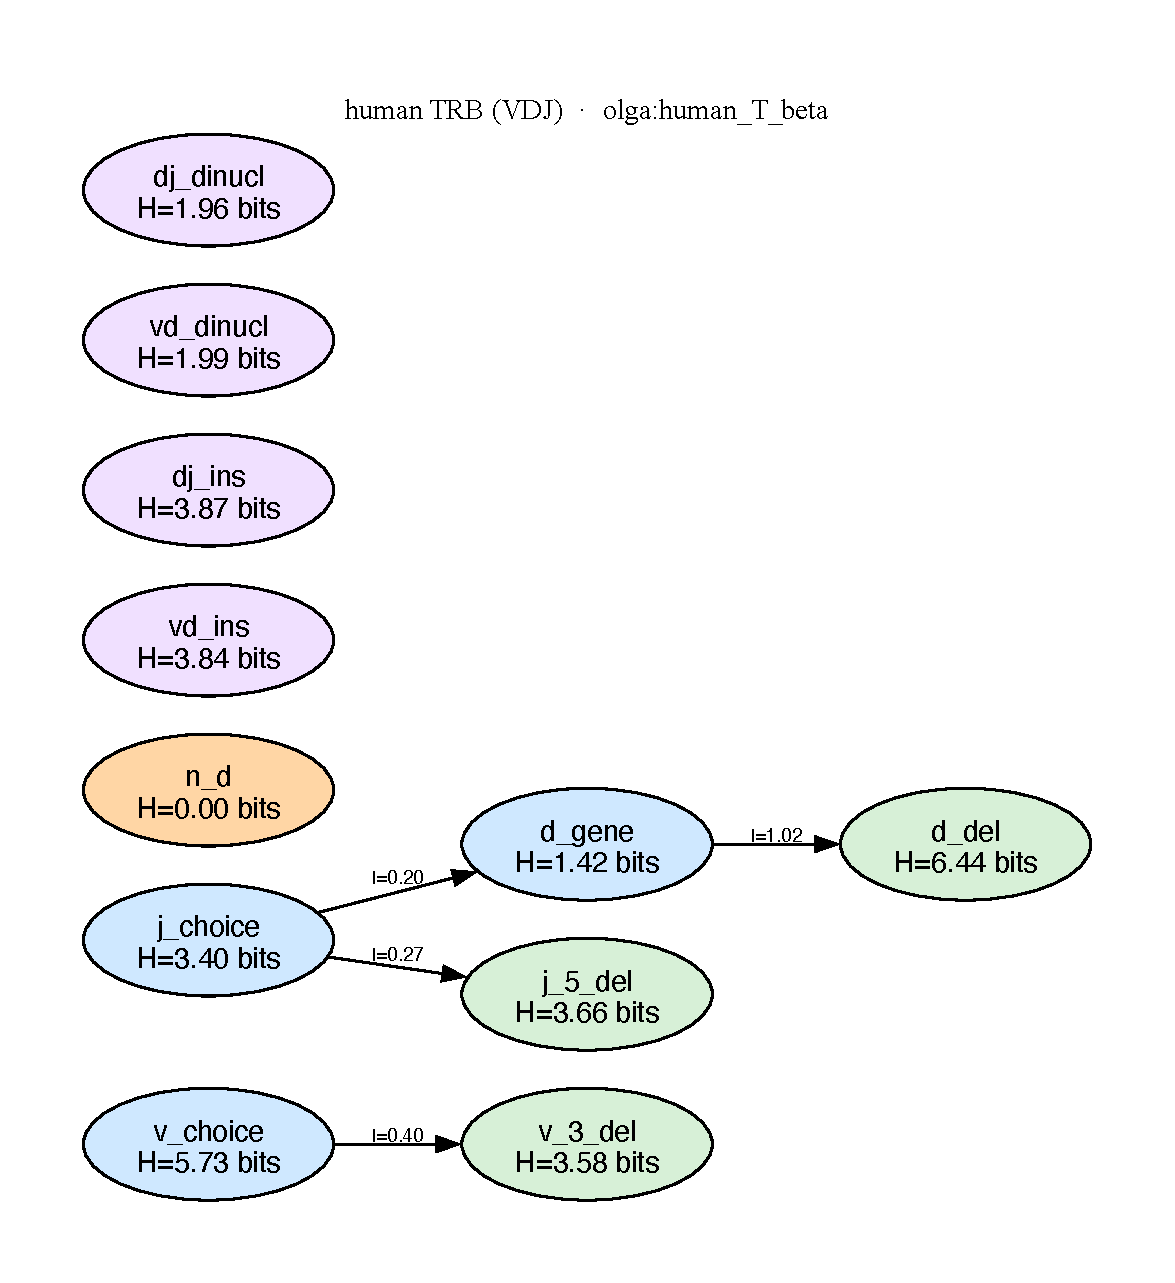
\includegraphics[width=0.49\linewidth]{bn_trb.pdf}\hfill
  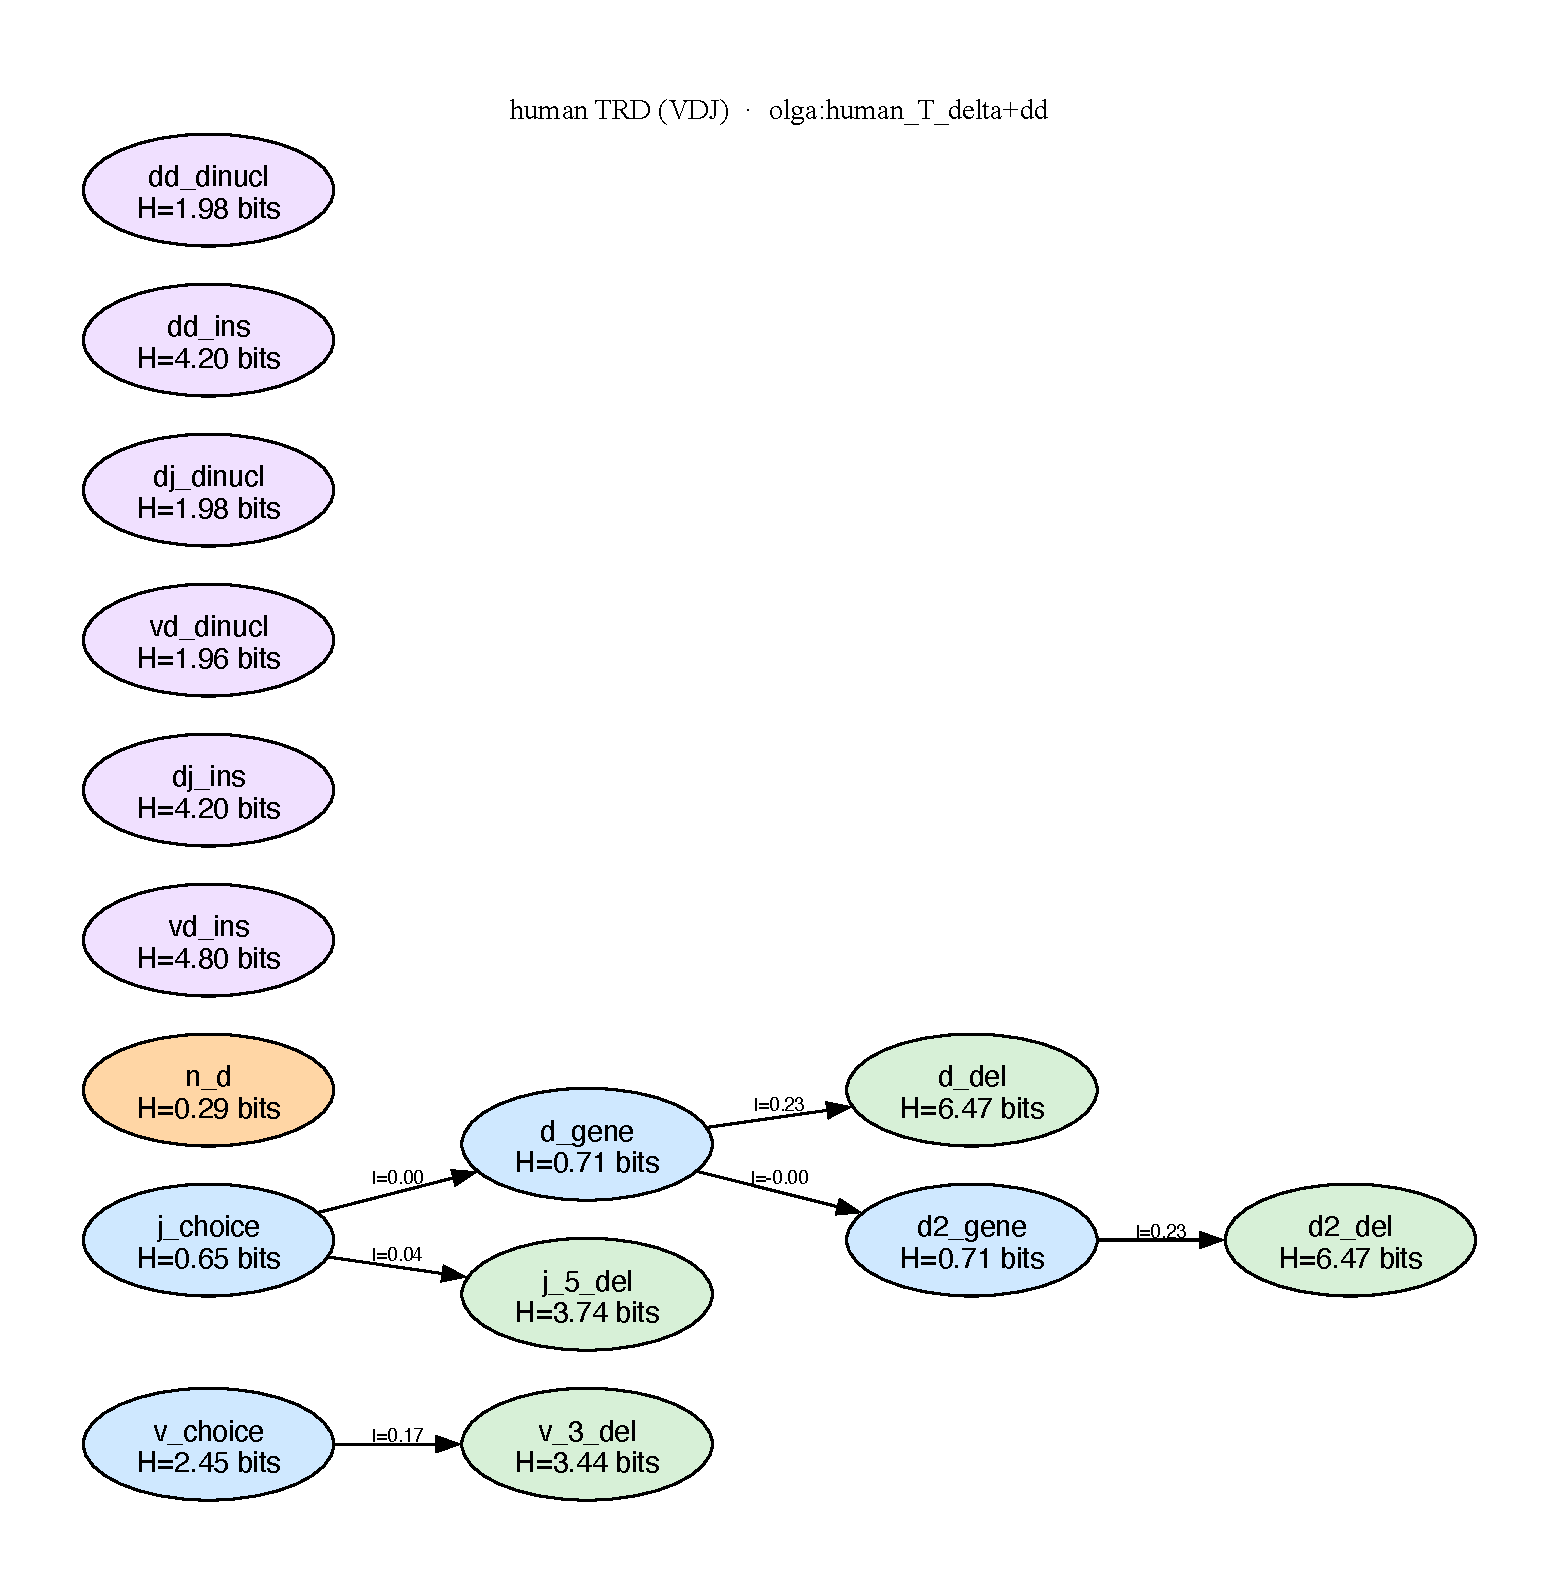
\includegraphics[width=0.49\linewidth]{bn_trd_dd.pdf}
  \caption{The recombination Bayesian network rendered from the manifest, nodes labelled with marginal
    entropy $H$ (bits) and edges with mutual information $I$ (bits). \emph{Left:} human TRB (single-$D$).
    \emph{Right:} human TRD upgraded to the tandem-$D$ model of \S\ref{sec:dd}, adding the $n_D$,
    $D_2$-gene, $D_2$-deletion and $DD$-insertion nodes.}
  \label{fig:bn}
\end{figure}

Table~\ref{tab:entropy} compares the per-event entropy across five loci; each row's most informative
locus is in bold. The structure is legible. Gene choice dominates in the $\alpha\beta$ loci ($H_V\!\approx\!5.7$
bits for TRB, $H_J\!\approx\!5.6$ for TRA), whereas TRD spends little on gene choice ($H_V\!=\!2.4$ bits,
few $\delta$ genes) and the most on non-templated insertion ($H_{VD}\!=\!4.8$ bits) --- the TdT signature.
The single most entropic event in every $VDJ$ locus is the joint $D$-deletion (up to $7.8$ bits for IGH),
and its two ends are far from independent: the within-$D$ coupling $I(\del_D^{5'};\del_D^{3'}\!\mid\!D)=1.18$
bits for TRB (a genuine conditional mutual information, averaged over $D$ so that the shared choice of $D$
does not inflate it). Two edges are worth naming. First, $I(V;J)=0$ for every $VDJ$ locus is not a
measurement but an \emph{assumption} made visible --- \texttt{OLGA} factors $P(V,J)=P(V)P(J)$ --- whereas
the $VJ$ loci carry $I(V;J)>0$ through $P(J\mid V)$ (e.g.\ $0.27$ bits for TRA). Second, the $D$-deletion
edge $I(\{\del_D\};D)$ is large
($1.02$ bits for TRB), i.e.\ trimming depends strongly on which $D$ was chosen. The identical routine
applies to an EM-inferred model, so the same table compares a model learned from real reads against the
\texttt{OLGA} bootstrap parameter-by-parameter. On $6000$ real out-of-frame human TRB clonotypes
(single-$D$ EM, aligned-gene mask; \texttt{bench\_em.py}) the fitted model places broader mass on
exonuclease deletion and non-templated insertion than the synthetic bootstrap --- the $D$-deletion
entropy rises from $6.44$ to $7.65$ bits and the $VD$-insertion entropy from $3.84$ to $4.50$ bits, while
the held-out log-likelihood improves --- i.e.\ real repertoires are less tightly trimmed and inserted than
the \texttt{OLGA} generative model, and the within-$D$ coupling stays near $1$ bit under both.

\begin{table}[t]
  \centering
  \small
  \caption{Marginal entropy $H(X)$ (bits) of each recombination event across five human loci, computed
    from the model tables. Dashes mark events absent from a locus ($VJ$ loci have no $D$; $\alpha\beta$
    loci no $VJ$ insertion). Bold marks the most entropic locus per event.}
  \label{tab:entropy}
  \begin{tabular}{lccccc}
    \toprule
    Event & TRB & TRA & TRD & IGH & IGK \\
    \midrule
    $V$ choice            & \textbf{5.73} & 5.37 & 2.45 & 5.71 & 4.81 \\
    $J$ choice            & 3.40 & \textbf{5.57} & 0.65 & 2.17 & 2.83 \\
    $D$ gene $\mid J$      & 1.42 & --- & 0.71 & \textbf{4.30} & --- \\
    $V\,3'$ deletion      & 3.58 & \textbf{3.69} & 3.44 & 3.46 & 3.15 \\
    $J\,5'$ deletion      & 3.66 & 3.89 & 3.74 & \textbf{4.13} & 3.65 \\
    $D$ deletion (5$'$,3$'$) & 6.44 & --- & 6.47 & \textbf{7.78} & --- \\
    $VD$ insertion length & 3.84 & --- & \textbf{4.80} & 4.68 & --- \\
    $DJ$ insertion length & 3.87 & --- & 4.20 & \textbf{4.82} & --- \\
    $VJ$ insertion length & --- & \textbf{3.84} & --- & --- & 3.59 \\
    $VD$ dinucleotide     & \textbf{1.99} & --- & 1.96 & 1.98 & --- \\
    $DJ$ dinucleotide     & 1.96 & --- & 1.98 & \textbf{1.99} & --- \\
    $VJ$ dinucleotide     & --- & \textbf{1.97} & --- & --- & 1.92 \\
    \bottomrule
  \end{tabular}
\end{table}

\bibliographystyle{unsrt}
\bibliography{refs}

\end{document}
